\hiddenappendixchapter
    {Secondary Implementation Improvements}
    {app:secondary_implementation_improvements}

\providecommand{\appBimage}[1]{%
    \IfFileExists{#1}{%
        \includegraphics[
            width=\linewidth,
            keepaspectratio
        ]{#1}%
    }{%
        \fbox{%
            \parbox[c][0.13\textheight][c]{0.92\linewidth}{%
                \centering
                \textbf{Capture pending}\\[0.6em]
                \texttt{\detokenize{#1}}
            }%
        }%
    }%
}

Several adaptations introduced during the development are secondary to the
transient and electrical methods described in the main chapters. They improve
selection consistency, temporal evaluation, conductor inspection, user
feedback, persistent storage and code organisation. The following sections
compare the relevant behaviour of the initial and final implementations and
document only functions present in the final application.

\section{Comparison of Initial and Final Behaviour}
\label{appsec:secondary_behaviour_comparison}

Table~\ref{tab:appendix_secondary_improvements} summarises the selected
adaptations. The comparison is based on the operation of both application
versions and on the final source-code organisation. It is not intended as a
complete change log, since the transient and electrical developments are
already described in Chapters~\ref{ch:multicase_tool},
\ref{ch:transient_analysis} and~\ref{ch:electrical_battery_analysis}.

% File: Tables/table_appendix_secondary_improvements.tex
\begingroup
\small
\renewcommand{\arraystretch}{1.12}
\setlength{\tabcolsep}{3pt}
\begin{longtable}{|>{\raggedright\arraybackslash}p{0.25\textwidth}|>{\raggedright\arraybackslash}p{0.35\textwidth}|>{\raggedright\arraybackslash}p{0.27\textwidth}|}
    \caption{Comparison of selected secondary implementation improvements.}
    \label{tab:appendix_secondary_improvements}\\
    \hline
    \textbf{Initial behaviour} & \textbf{Final behaviour} & \textbf{Main location} \\
    \hline
    \endfirsthead

    \multicolumn{3}{c}{\tablename\ \thetable\ -- continued}\\
    \hline
    \textbf{Initial behaviour} & \textbf{Final behaviour} & \textbf{Main location} \\
    \hline
    \endhead

    \hline
    \endfoot

    Group selectors were not consistently ordered according to the model
    structure. &
    Available groups follow the parent--child order defined by the Excel
    hierarchy, with fallback ordering for malformed or disconnected branches. &
    Common hierarchy-selection helpers and inherited group selectors. \\
    \hline
    Parent and descendant groups could be selected together and counted twice
    in aggregated results. &
    Descendants already included in a selected parent are removed and a visible
    message identifies the corrected selection. &
    Flow Explorer and compatible hierarchical selectors. \\
    \hline
    Several inherited modules evaluated only the active or first stored output
    state. &
    The selected value from the result-file time vector is applied to each
    compatible calculation and retained when the analysis is restored. &
    Flow Explorer, Group Attributes, GL/GR Conductors, Nodes and Group Study. \\
    \hline
    GL and GR inspection focused on individual source--target tables. &
    The final tabs also provide matrix-quality summaries, configurable high and
    low thresholds and detailed issue tables. &
    GL Conductors and GR Conductors. \\
    \hline
    Nodal filtering was applied while the filter text was being entered. &
    Separate \textit{Apply filter} and \textit{Clear filter} controls preserve
    an explicit active-filter state. &
    Nodes. \\
    \hline
    Interface candidates could be selected from hierarchy groups without
    confirming an explicit thermal connection. &
    GL and GR definitions are scanned to identify connected target groups and
    node pairs before the interface calculation. &
    Transient interface analysis. \\
    \hline
    Temperature changes over prescribed time intervals were not available as a
    complete analysis area. &
    Maximum and minimum temperature changes are calculated over selectable
    10-, 15-, 30- and 60-minute windows and summarised by group. &
    Transient temperature-variation analysis. \\
    \hline
    Validation and feedback differed between individual interface blocks. &
    Missing cases, empty selections and unavailable data produce visible
    messages before the calculation continues. &
    All final analysis modules. \\
    \hline
    Saving logic was distributed among individual output areas. &
    Saved analyses share a common database, file store, restoration recipe and
    editing workflow. &
    Scene-management and restoration modules. \\
    \hline
    Most interface areas were concentrated in the main application script. &
    The launcher, analysis tabs, shared helpers and persistence functions are
    separated into dedicated modules. &
    Application architecture. \\
    \hline
\end{longtable}
\endgroup


\section{Hierarchy Safeguards and Time-Dependent Inspection}
\label{appsec:hierarchy_time_safeguards}

Hierarchy-aware selection prevents the same physical branch from being
included more than once in an aggregated result. Figure~
\ref{fig:appendix_hierarchy_warning} shows the message produced when a parent
group and one or more of its descendants are selected simultaneously. The
descendants are removed because their nodes are already contained in the
parent selection.

\begin{figure}[!htbp]
    \centering
    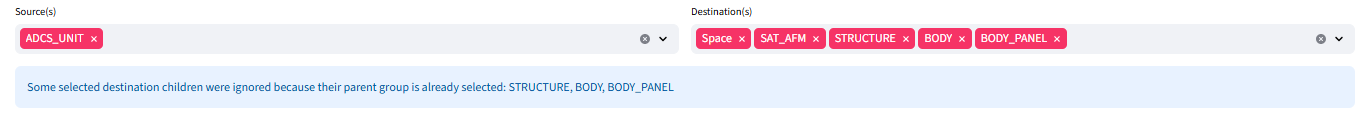
\includegraphics[
        width=0.94\textwidth,
        keepaspectratio
    ]{Figures/Anexo_02/hierarchy_selection_warning.png}
    \caption{Automatic removal of redundant descendant groups.}
    \label{fig:appendix_hierarchy_warning}
\end{figure}

The inherited modules use the output-time vector stored in each transient
result file. The selected instant is evaluated independently in each tab so
that its configuration can be saved and restored together with the remaining
controls. Table~\ref{tab:appendix_time_dependent_modules} identifies the
result evaluated at that instant.

% File: Tables/table_appendix_time_dependent_modules.tex
\begin{table}[H]
    \centering
    \caption{Use of the selected output time in the inherited modules.}
    \label{tab:appendix_time_dependent_modules}
    \small
    \renewcommand{\arraystretch}{1.13}
    \setlength{\tabcolsep}{3pt}
    \begin{tabularx}{\textwidth}{|>{\raggedright\arraybackslash}p{0.18\textwidth}|>{\raggedright\arraybackslash}X|>{\raggedright\arraybackslash}X|}
        \hline
        \textbf{Module} & \textbf{Time-dependent output} & \textbf{Stored setting} \\
        \hline
        Flow Explorer &
        Instantaneous source--target heat flows used by the selected graph. &
        Output time, groups, units, tolerance and graph type. \\
        \hline
        Group Attributes &
        Group temperatures, thermal loads and selected metadata. &
        Output time, cases, groups, attributes and representation mode. \\
        \hline
        GL Conductors &
        Linear-conductor values between the selected source and target. &
        Output time, groups and case selection. \\
        \hline
        GR Conductors &
        Radiative-conductor values between the selected source and target. &
        Output time, groups and case selection. \\
        \hline
        Nodes &
        Nodal temperatures, loads and selected node attributes. &
        Output time, cases, groups, attributes and active filter. \\
        \hline
        Group Study &
        Group summary and internal or external conductor values. &
        Output time, case, group, conductor type and units. \\
        \hline
    \end{tabularx}
\end{table}


Figure~\ref{fig:appendix_time_controls} provides two representative examples.
The Group Attributes selector is populated from the transient result vector,
whereas the GL tab uses the chosen time when generating the conductor table.
Equivalent controls are used by the remaining compatible modules.

\begin{figure}[H]
    \centering

    \begin{subfigure}[t]{0.48\textwidth}
        \centering
        \appBimage{Figures/Anexo_02/time_control_group_attributes.png}
        \caption{Group Attributes.}
        \label{fig:appendix_time_group_attributes}
    \end{subfigure}
    \hfill
    \begin{subfigure}[t]{0.48\textwidth}
        \centering
        \appBimage{Figures/Anexo_02/time_control_gl_conductors.png}
        \caption{GL Conductors.}
        \label{fig:appendix_time_gl_conductors}
    \end{subfigure}

    \caption{Representative output-time controls in inherited modules.}
    \label{fig:appendix_time_controls}
\end{figure}

\FloatBarrier

\section{Conductor Inspection and Interface Detection}
\label{appsec:conductor_interface_detection}

The GL and GR tabs include matrix-level diagnostics in addition to the
source--target tables described in Appendix~
\ref{app:inherited_interface_evolution}. The summaries report the number of
couplings and classify values according to configurable high and low
thresholds. Detailed issue tables can then isolate the affected pairs and be
saved independently.

\begin{figure}[!htbp]
    \centering

    \begin{subfigure}[t]{0.48\textwidth}
        \centering
        \appBimage{Figures/Anexo_02/gl_matrix_quality_summary.png}
        \caption{GL matrix summary.}
        \label{fig:appendix_gl_matrix_summary}
    \end{subfigure}
    \hfill
    \begin{subfigure}[t]{0.48\textwidth}
        \centering
        \appBimage{Figures/Anexo_02/gr_matrix_quality_summary.png}
        \caption{GR matrix summary.}
        \label{fig:appendix_gr_matrix_summary}
    \end{subfigure}

    \caption{Matrix-quality summaries available in the conductor tabs.}
    \label{fig:appendix_conductor_matrix_summaries}
\end{figure}

The transient interface analysis uses the same explicit connection data to
restrict the destination selector when the conductor filter is active. Only
node pairs connected through GL or GR definitions are evaluated. The
hierarchy remains available as a fallback when no explicit target is detected.

\begin{figure}[!htbp]
    \centering
    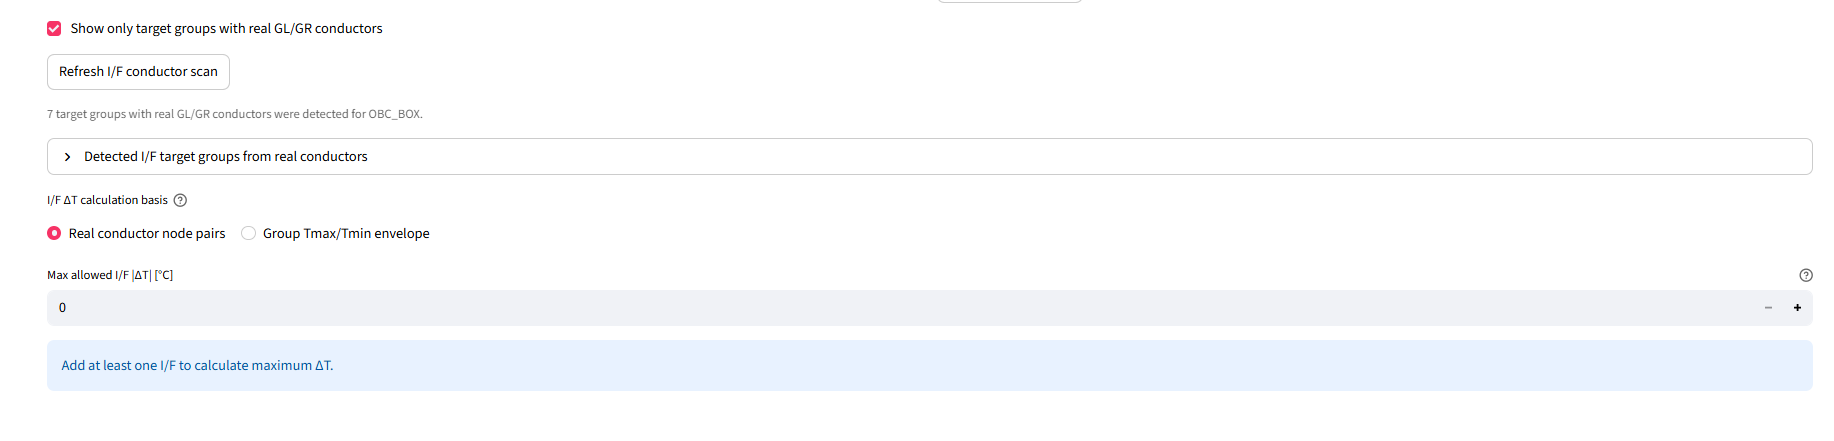
\includegraphics[
        width=0.94\textwidth,
        keepaspectratio
    ]{Figures/Anexo_02/interface_conductor_filter.png}
    \caption{Conductor-based filtering of candidate interface groups.}
    \label{fig:appendix_interface_conductor_filter}
\end{figure}

Table~\ref{tab:appendix_obc_detected_targets} provides a numerical example for
\texttt{OBC\_BOX}. The target groups and pair counts are obtained from the
same connection scan used to populate the interface selector. The table
documents the connection basis applied before the temperature differences are
calculated.

% File: Tables/table_appendix_obc_detected_targets.tex
% Usage: \AppendixOBCDetectedTargetsTable[0.94\textwidth]

\newcommand{\AppendixOBCDetectedTargetsTable}[1][0.94\textwidth]{%
\begin{table}[!htbp]
    \centering
    \caption{Target groups detected from the explicit GL and GR connections
    to \texttt{OBC\_BOX} in the nominal case.}
    \label{tab:appendix_obc_detected_targets}
    \renewcommand{\arraystretch}{1.16}
    \setlength{\tabcolsep}{4pt}
    \resizebox{#1}{!}{%
    \begin{tabular}{@{}lrrrrr@{}}
        \toprule
        \textbf{Target group} &
        \textbf{GL pairs} &
        \textbf{$\sum |GL|$ [W/K]} &
        \textbf{GR pairs} &
        \textbf{$\sum |GR|$ [m$^2$]} &
        \textbf{Total pairs} \\
        \midrule
        \texttt{BODY} & 4 & 22.68 & 559 & 0.355732 & 563 \\
        \texttt{RADIATOR} & 4 & 0.40 & 181 & 0.020584 & 185 \\
        \texttt{BODY\_PLATE\_MED} & 4 & 22.68 & 96 & 0.115546 & 100 \\
        \texttt{BODY\_PANEL} & 0 & 0.00 & 364 & 0.147134 & 364 \\
        \texttt{BODY\_PLATE\_SUP} & 0 & 0.00 & 91 & 0.092968 & 91 \\
        \texttt{Space} & 0 & 0.00 & 24 & 0.001042 & 24 \\
        \texttt{BODY\_PLATE\_INF} & 0 & 0.00 & 8 & 0.000083 & 8 \\
        \bottomrule
    \end{tabular}%
    }
\end{table}%
}

\AppendixOBCDetectedTargetsTable[0.94\textwidth]

\FloatBarrier

\section{Input Validation and User Feedback}
\label{appsec:validation_feedback}

The final interface checks the information required by each calculation before
processing begins. Missing cases, empty group selections, unsupported
combinations and unavailable conductor data produce visible messages instead
of incomplete outputs or uncaught errors. Figure~
\ref{fig:appendix_validation_no_case} shows the response when no case has been
selected. Equivalent checks are applied locally by the remaining modules.

\begin{figure}[!htbp]
    \centering
    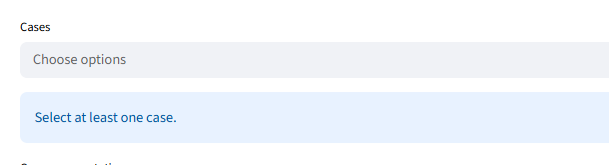
\includegraphics[
        width=0.72\textwidth,
        keepaspectratio
    ]{Figures/Anexo_02/validation_no_case.png}
    \caption{Validation message displayed when no case is selected.}
    \label{fig:appendix_validation_no_case}
\end{figure}

\section{Persistent Analysis Storage}
\label{appsec:persistent_analysis_storage}

The saving workflow described in Section~\ref{sec:analysis_saving_export}
uses an SQLite database together with a structured file store. The database
relates each saved analysis to its model, cases, source tab, model element and
stored recipe. The file directory contains the generated representations and
a JSON description of the settings required for restoration.

A saved entry follows the general structure below. The exact intermediate
folders depend on whether the output belongs to one case, several cases or a
case-difference comparison.

\begin{lstlisting}[basicstyle=\ttfamily\small, frame=single]
scene_store/
+-- <model>/
    +-- <scope_and_cases>/
        +-- <element_type>_<element>/
            +-- scene_<timestamp>_<tab>_<name>/
                +-- scene.json
                +-- figure.plotly.json
                +-- figure.html
                +-- table.csv
                +-- table.xlsx
                +-- figure.png
                +-- figure.svg
\end{lstlisting}

Only the files associated with the generated output are created. Plotly
figures produce JSON and HTML files, data tables produce CSV and spreadsheet
files, and Matplotlib figures produce PNG and SVG images. The metadata file is
always written.

% File: Tables/table_appendix_saved_analysis_artifacts.tex
\begin{table}[!htbp]
    \centering
    \caption{Files and records associated with a saved analysis.}
    \label{tab:appendix_saved_analysis_artifacts}
    \small
    \renewcommand{\arraystretch}{1.14}
    \setlength{\tabcolsep}{4pt}
    \begin{tabularx}{\textwidth}{|>{\raggedright\arraybackslash}p{0.26\textwidth}|>{\raggedright\arraybackslash}X|}
        \hline
        \textbf{Stored item} & \textbf{Purpose} \\
        \hline
        SQLite model, case and analysis records &
        Relate the saved output to its source files, visible case names,
        element, tab and creation metadata. \\
        \hline
        Recipe JSON in the database &
        Stores widget values required to restore the analysis configuration. \\
        \hline
        \texttt{scene.json} &
        Provides a readable file copy of the saved metadata and recipe. \\
        \hline
        \texttt{figure.plotly.json} and \texttt{figure.html} &
        Preserve an interactive Plotly figure and provide an independent
        browser representation. \\
        \hline
        \texttt{table.csv} and \texttt{table.xlsx} &
        Preserve a generated numerical table in two conventional formats. \\
        \hline
        \texttt{figure.png} and \texttt{figure.svg} &
        Preserve a Matplotlib figure for reports and scalable editing. \\
        \hline
    \end{tabularx}
\end{table}


Consistency checks remove database entries whose folders no longer exist and
scene folders that are no longer referenced by the database. An auxiliary
cleanup script creates backups before removing saved analyses unrelated to a
defined set of retained model files. These functions reduce stale references
without changing the original \texttt{.TMD} or hierarchy files.

\section{Source-Code Reorganisation}
\label{appsec:source_code_reorganisation}

The initial interface concentrates the inherited tabs in a single application
script. The final organisation separates each analysis area from the launcher
and isolates saving and restoration functions in dedicated modules. This
structure allows one tab to be modified without rewriting the complete
interface and supports the addition of the transient and electrical modules.

% File: Tables/table_appendix_code_reorganisation.tex
\begingroup
\footnotesize
\renewcommand{\arraystretch}{1.06}
\setlength{\tabcolsep}{3pt}
\begin{longtable}{|>{\raggedright\arraybackslash}p{0.32\textwidth}|>{\raggedright\arraybackslash}p{0.58\textwidth}|}
    \caption{Correspondence between the initial interface blocks and the final modules.}
    \label{tab:appendix_code_reorganisation}\\
    \hline
    \textbf{Initial block} & \textbf{Final module} \\
    \hline
    \endfirsthead

    \multicolumn{2}{c}{\tablename\ \thetable\ -- continued}\\
    \hline
    \textbf{Initial block} & \textbf{Final module} \\
    \hline
    \endhead

    \hline
    \endfoot

    Flow Explorer block in \texttt{app\_interactiva.py} &
    \texttt{tabs/tab\_flow\_explorer.py} \\
    \hline
    Model-information block &
    \texttt{tabs/tab\_case\_info.py} \\
    \hline
    Group-attribute block &
    \texttt{tabs/tab\_group\_attributes.py} \\
    \hline
    GL and GR blocks &
    \texttt{tabs/tab\_gl\_conductors.py} and
    \texttt{tabs/tab\_gr\_conductors.py} \\
    \hline
    Nodes and group-study blocks &
    \texttt{tabs/tab\_nodes.py} and
    \texttt{tabs/tab\_group\_study.py} \\
    \hline
    Initial transient prototype &
    \texttt{tabs/tab\_transient.py} \\
    \hline
    Solar and battery calculations &
    \texttt{tabs/tab\_sp.py} \\
    \hline
    Saving and restoration functions &
    \texttt{app\_thermalviewer/scene\_manager.py},
    \texttt{scene\_ui.py}, \texttt{restored\_scenes.py} and
    \texttt{scene\_editor.py} \\
    \hline
    Common widget, hierarchy and export routines &
    \texttt{app\_thermalviewer/app\_helpers.py} and
    \texttt{viewer\_utils.py} \\
    \hline
\end{longtable}
\endgroup


The reorganisation changes only the software structure; all modules continue
to share the same imported case and hierarchy objects.

\FloatBarrier
